
% Template for Elsevier CRC journal article
% version 1.2 dated 09 May 2011

% This file (c) 2009-2011 Elsevier Ltd.  Modifications may be freely made,
% provided the edited file is saved under a different name

% This file contains modifications for Procedia Computer Science
% but may easily be adapted to other journals

% Changes since version 1.1
% - added "procedia" option compliant with ecrc.sty version 1.2a
%   (makes the layout approximately the same as the Word CRC template)
% - added example for generating copyright line in abstract

%-----------------------------------------------------------------------------------

%% This template uses the elsarticle.cls document class and the extension package ecrc.sty
%% For full documentation on usage of elsarticle.cls, consult the documentation "elsdoc.pdf"
%% Further resources available at http://www.elsevier.com/latex

%-----------------------------------------------------------------------------------

%%%%%%%%%%%%%%%%%%%%%%%%%%%%%%%%%%%%%%%%%%%%%%%%%%%%%%%%%%%%%%
%%%%%%%%%%%%%%%%%%%%%%%%%%%%%%%%%%%%%%%%%%%%%%%%%%%%%%%%%%%%%%
%%                                                          %%
%% Important note on usage                                  %%
%% -----------------------                                  %%
%% This file should normally be compiled with PDFLaTeX      %%
%% Using standard LaTeX should work but may produce clashes %%
%%                                                          %%
%%%%%%%%%%%%%%%%%%%%%%%%%%%%%%%%%%%%%%%%%%%%%%%%%%%%%%%%%%%%%%
%%%%%%%%%%%%%%%%%%%%%%%%%%%%%%%%%%%%%%%%%%%%%%%%%%%%%%%%%%%%%%

%% The '3p' and 'times' class options of elsarticle are used for Elsevier CRC
%% Add the 'procedia' option to approximate to the Word template
%\documentclass[3p,times,procedia]{elsarticle}
\documentclass[3p,times]{elsarticle}
\usepackage{natbib}
\usepackage{graphicx}
\usepackage{listings}
\usepackage{amsmath}
\usepackage{url}
\usepackage{color}
\definecolor{lightgray}{rgb}{.7,.7,.7}
\definecolor{gray}{rgb}{.4,.4,.4}
\definecolor{darkblue}{rgb}{0,0,.3}
\lstset{
	  basicstyle=\ttfamily,
	    columns=fullflexible,
		  showstringspaces=false,
		    commentstyle=\color{gray}\upshape
		}

		\lstdefinelanguage{XML}
		{
			  morestring=[b]",
			    morestring=[s]{>}{<},
				  morecomment=[s]{<?}{?>},
				    stringstyle=\color{black},
					  identifierstyle=\color{darkblue},
					    keywordstyle=\color{cyan},
						  morekeywords={xmlns,version,type, action}% list your attributes here
					  }
%% The `ecrc' package must be called to make the CRC functionality available
\usepackage{ecrc}

%% The ecrc package defines commands needed for running heads and logos.
%% For running heads, you can set the journal name, the volume, the starting page and the authors

%% set the volume if you know. Otherwise `00'
\volume{00}

%% set the starting page if not 1
\firstpage{1}

%% Give the name of the journal
\journalname{Computer Communications}

%% Give the author list to appear in the running head
%% Example \runauth{C.V. Radhakrishnan et al.}
\runauth{Dustin Wright and Yusuf Ozturk}

%% The choice of journal logo is determined by the \jid and \jnltitlelogo commands.
%% A user-supplied logo with the name <\jid>logo.pdf will be inserted if present.
%% e.g. if \jid{yspmi} the system will look for a file yspmilogo.pdf
%% Otherwise the content of \jnltitlelogo will be set between horizontal lines as a default logo

%% Give the abbreviation of the Journal.  Contact the journal editorial office if in any doubt
\jid{comcom}

%% Give a short journal name for the dummy logo (if needed)
\jnltitlelogo{Computer Communications}

%% Provide the copyright line to appear in the abstract
%% Usage:
%   \CopyrightLine[<text-before-year>]{<year>}{<restt-of-the-copyright-text>}
%   \CopyrightLine[Crown copyright]{2011}{Published by Elsevier Ltd.}
%   \CopyrightLine{2011}{Elsevier Ltd. All rights reserved}
\CopyrightLine{2014}{Published by Elsevier Ltd.}

%% Hereafter the template follows `elsarticle'.
%% For more details see the existing template files elsarticle-template-harv.tex and elsarticle-template-num.tex.

%% Elsevier CRC generally uses a numbered reference style
%% For this, the conventions of elsarticle-template-num.tex should be followed (included below)
%% If using BibTeX, use the style file elsarticle-num.bst

%% End of ecrc-specific commands
%%%%%%%%%%%%%%%%%%%%%%%%%%%%%%%%%%%%%%%%%%%%%%%%%%%%%%%%%%%%%%%%%%%%%%%%%%

%% The amssymb package provides various useful mathematical symbols
\usepackage{amssymb}
%% The amsthm package provides extended theorem environments
%% \usepackage{amsthm}

%% The lineno packages adds line numbers. Start line numbering with
%% \begin{linenumbers}, end it with \end{linenumbers}. Or switch it on
%% for the whole article with \linenumbers after \end{frontmatter}.
%% \usepackage{lineno}

%% natbib.sty is loaded by default. However, natbib options can be
%% provided with \biboptions{...} command. Following options are
%% valid:

%%   round  -  round parentheses are used (default)
%%   square -  square brackets are used   [option]
%%   curly  -  curly braces are used      {option}
%%   angle  -  angle brackets are used    <option>
%%   semicolon  -  multiple citations separated by semi-colon
%%   colon  - same as semicolon, an earlier confusion
%%   comma  -  separated by comma
%%   numbers-  selects numerical citations
%%   super  -  numerical citations as superscripts
%%   sort   -  sorts multiple citations according to order in ref. list
%%   sort&compress   -  like sort, but also compresses numerical citations
%%   compress - compresses without sorting
%%
%% \biboptions{comma,round}

% \biboptions{}

% if you have landscape tables
\usepackage[figuresright]{rotating}

% put your own definitions here:
%   \newcommand{\cZ}{\cal{Z}}
%   \newtheorem{def}{Definition}[section]
%   ...

% add words to TeX's hyphenation exception list
%\hyphenation{author another created financial paper re-commend-ed Post-Script}

% declarations for front matter

\begin{document}

\begin{frontmatter}

%% Title, authors and addresses

%% use the tnoteref command within \title for footnotes;
%% use the tnotetext command for the associated footnote;
%% use the fnref command within \author or \address for footnotes;
%% use the fntext command for the associated footnote;
%% use the corref command within \author for corresponding author footnotes;
%% use the cortext command for the associated footnote;
%% use the ead command for the email address,
%% and the form \ead[url] for the home page:
%%
%% \title{Title\tnoteref{label1}}
%% \tnotetext[label1]{}
%% \author{Name\corref{cor1}\fnref{label2}}
%% \ead{email address}
%% \ead[url]{home page}
%% \fntext[label2]{}
%% \cortext[cor1]{}
%% \address{Address\fnref{label3}}
%% \fntext[label3]{}

%%\dochead{}
%% Use \dochead if there is an article header, e.g. \dochead{Short communication}
%% \dochead can also be used to include a conference title, if directed by the editors
%% e.g. \dochead{17th International Conference on Dynamical Processes in Excited States of Solids}

\title{UDAB-ViS: User Driven Adaptable Bandwidth Video System}

%% use optional labels to link authors explicitly to addresses:
%% \author[label1,label2]{<author name>}
%% \address[label1]{<address>}
%% \address[label2]{<address>}

\author{Dustin Wright and Yusuf Ozturk}

\address{5500 Campanile Dr. San Diego, California 92182}

\begin{abstract}
Adaptive bitrate (ABR) streaming has become an important and prevalent feature in many multimedia delivery systems, with content providers such as Netflix and Amazon using ABR streaming to increase bandwidth efficiency and provide the maximum user experience when channel conditions are not ideal. Where such systems could see improvement is in the delivery of live video with a closed loop cognitive control of video encoding. In this research, we present a camera system which provides spatially and temporally adaptive video streams, learning the user’s preferences in order to make intelligent scaling decisions. The system employs a hardware H.264/AVC encoder for video compression. The encoding parameters can be configured by the user or by the cognitive system on behalf of the user when the bandwidth changes. The cognitive video client  developed in this study learns the user’s preferences (i.e. video size over frame rate) over time and intelligently adapts  encoding parameters when the channel conditions change. It has been demonstrated that the cognitive decision system developed has  the ability to control video bandwidth by altering the spatial and temporal resolution, as well as the ability to make scaling decisions .
\end{abstract}

\begin{keyword}
%% keywords here, in the form: keyword \sep keyword
Video Streaming \sep H.264 \sep Machine Learning \sep Bandwidth
%% PACS codes here, in the form: \PACS code \sep code

%% MSC codes here, in the form: \MSC code \sep code
%% or \MSC[2008] code \sep code (2000 is the default)

\end{keyword}

\end{frontmatter}

%%
%% Start line numbering here if you want
%%
% \linenumbers

%% main text
%%%%%%%%%%%%%%%%%%%%%%%%%%%%%%%%%%%%%%%%%%%%%%%%%%%%%%%%%%

\section{Introduction}
\label{sec:Intro}

As wireless networks become more ubiquitous and the number of devices capable of accessing these networks increases, the need for more efficient video streaming solutions becomes vastly important. By 2015, it is expected that approximately 90 percent of online consumer traffic and almost 66 percent of mobile traffic will be video \cite{HASQoE}. With increasing amount of video traffic, bandwidth efficiency becomes a serious concern in order to deliver the best quality of experience (QoE) to each individual user. At the same time, servers should be able to deliver video in such a way that information the user deems important is not lost due to bandwidth constraints and the method by which the video adapts.

To date, numerous solutions have been developed that take a range of approaches to solve this problem. Many of these approaches are based on already existing protocols such as the Real-Time Streaming Protocol RTSP \cite{RTSP}, TCP, and HTTP \cite{HASQoE, Apple, Microsoft, Netflix} and achieve bandwidth adaptability in one of a few ways. These bandwidth adaptability techniques include progressive download, adaptive bitrate (ABR) streaming, and stream-switching \cite{FeedbackControl}. In progressive download, video is transmitted as regular data files using TCP and is buffered by the client; playing starts when a sufficient amount of buffering has been achieved. This technique is employed by the popular video streaming website YouTube. Other solutions such as Netflix and Amazon Video employ ABR, in which the server can select the encoding bitrate in order to maximize the video quality for a given channel. The result is a drastic reduction in the need for buffering; from the end user's perspective, the quality resolution of the video changes as network conditions change. Finally, with stream switching, the server encodes the source video with different encoding parameters and allows the client to switch between streams based on network conditions. Examples of stream switching solutions can be found in \cite{FeedbackControl},\cite{Apple} and \cite{Microsoft}. Such techniques are ideal for online video streaming as they can use HTTP to negotiate streaming parameters and transmit the video stream; however, the major pitfall is that in most cases, only the video bitrate will be affected and no control is exercised over the spatial and temporal resolution of the video. In the case where spatial and temporal resolution can be affected, raw video will have to be re-encoded or transcoded at the source which can cause a delay in the video being transmitted \cite{FeedbackControl}.

In addition to protocol based approaches which tend to only allow for bitrate scalability, many codec based approaches have been developed which allow for easy spatial and temporal scalability \cite{SVCAdvances}. Two prime examples of codec based approaches are H.264/AVC and H.264/SVC \cite{SVCOverview}\cite{SVCTutorial}. With these codecs, video need only be encoded once and, due to the nature of the decoders, can be transmitted as several sub-streams in order to control the temporal or spatial resolution. The primary issue with this approach is that it limits the client to only a certain set of video decoders. A review of the H.264/SVC approach to scalability will be presented later in this paper.

A problem with many of these solutions is that only quality resolution is affected in order to control the video bandwidth, which may not be preferred in many applications. Numerous popularly used streaming solutions such as HTTP Adaptive Streaming (HAS) \cite{HASQoE} and Dynamic Adaptive Streaming over HTTP (DASH) \cite{DASH},  will throttle the bitrate of a video stream in order to adapt to changes in channel bandwidth, which will result in a change in video quality. This behavior is exhibited by the widely used video content provider Netflix, which employs DASH (and thus ABR) to achieve bandwidth adaptability \cite{Netflix}. A prime example where this system will not be viable is in medical teleconferencing. A patient may wish to have a remote consultation with his or her doctor in order to quickly and efficiently receive feedback about a medical problem such as a burn or lesion they may have endured. Were the video bandwidth to be controlled by ABR and the quality resolution be affected in order to fit to the channel, the doctor may not be able to properly diagnose or provide valid feedback to the user because the visual quality is not sufficient. However, if the system were to scale the temporal resolution of the video instead of the quality, visual information would be kept intact and the less important temporal information would be sacrificed. The system we developed uses this kind of scalability in tandem with the generation of user profiles in order to make an intelligent determination of how to alter each resolution. In this approach, video context is taken into consideration to provide different video scalability options in different situations. This addresses the issue of how to control the different encoding parameters in such a way as to align with the user’s desires without requiring the user to change the parameters themself.

One of the key factors to achieve such a system is the automation of video bandwidth control. In \cite{FeedbackControl}, the authors propose a \emph{Quality Adaptation Controller} which uses a proportional integrator (PI) controller at the server to select an appropriate video stream for the client. The system uses stream switching and employs feedback control to maintain the video bandwidth below the available channel bandwidth. This system succeeds in being a codec independent solution that is able to keep the video bandwidth at or below the available bandwidth with a transient time of less than 30 seconds, and is able to share the channel with concurrent streams \cite{FeedbackControl}. However, the solution does not take into account the context of the video and the user’s desires in order to select encoding parameters in an intelligent fashion. In this study, a learning module using support vector machines (SVM) has been created which learns the user’s preferences and is able to adapt the video appropriately. These preferences are learned based on contextual video features such as channel bandwidth and video content type, thus allowing for different functionality in different situations.

The rest of the paper is structured as follows; in section \ref{sec:Packetization} we review H.264 packetization. In section \ref{sec:SVC}, we review H.264/SVC as a scalable streaming solution, as well as the scalability solution used in our system. Sections \ref{sec:Architecture} and \ref{sec:Snapdragon} will describe the system architecture proposed in this study, as well as the method by which the video is encoded. Section \ref{sec:UserProfiles} will detail our learning model and how video bandwidth is optimized. Finally, test setup and experimental results will be presented in section \ref{sec:Results}.

%%%%%%%%%%%%%%%%%%%%%%%%%%%%%%%%%%%%%%%%%%%%%%%%%%%%%%%%%%

\section{Packetization and Frame Encoding for H.264}
\label{sec:Packetization}

\subsection{H.264/AVC Basics}

H.264/AVC is a video coding standard developed jointly by the ITU-T Video Coding Experts Group (VCEG) and ISO/IEC Moving Pictures Expert Group (MPEG) designed with the goals of enhanced video compression and ``network friendly'' video representation addressing ``conversational'' applications such as video conferencing, as well as ``non-conversational'' applications such as broadcast streaming \cite{H264AVCOverview}. In December of 2001 VCEG and MPEG formed a Joint Video Team (JVT) which in March of 2003 finalized the draft of the H.264/AVC video coding standard for formal submission \cite{H264AVCOverview}. 

The standard provides highly efficient video coding and can be used in a breadth of applications, from storage to streaming. It provides bitrate savings of 50\% or more over its predecessor video codecs \cite{RTP}. This makes H.264/AVC especially applicable in wireless environments. The effectiveness of H.264/AVC as a tool for video compression over IP networks and in wireless settings is reviewed  in \cite{H264OverIP} and \cite{WirelessH264}. In addition, H.264 employs a litany of features to enhance the quality and customization of video coding. Some examples of these features are 
\begin{itemize}
	\item Motion vectors over picture boundaries
	\item Multiple reference picture motion compensation: P-frames and B-frames can select from a large number of stored reference pictures to determine the values in the current frame \cite{H264AVCOverview}
	\item Weighted prediction
\end{itemize}
In addition, H.264/AVC supports a number of features to allow greater error resilience and flexibility over many environments \cite{H264AVCOverview}. Some of these important features are
\begin{itemize}
	\item NAL unit syntax structure
	\item Flexible slice size
	\item Flexible Macroblock Ordering (FMO)
	\item Arbitrary Slice Ordering
\end{itemize}
 \cite{H264AVCOverview} and \cite{H264Spec} provide a detailed overview of each of these features. The structure of an H.264/AVC encoder is depicted in Figure \ref{fig:H264EncoderStructure}.
\begin{figure}[h]
\centering
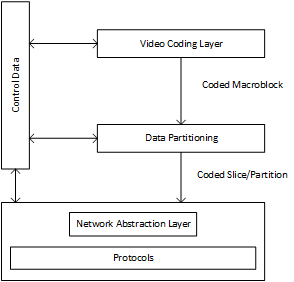
\includegraphics[width=0.4\linewidth]{H264AVCEncoderStructure.png}
\caption{H.264/AVC Encoder Structure \cite{H264AVCOverview}}
\label{fig:H264EncoderStructure}
\end{figure}
The codec given in Figure \ref{fig:H264EncoderStructure} covers both the Video Coding Layer (VCL) and the Network Abstraction Layer (NAL). The VCL performs the physical encoding and compression of video while the NAL adds a header to video packet data and is exceptionally important to assist the decoder in understanding how to handle the packetized frames. We will now discuss the NAL and give a general overview of how frames are packetized when sent over UDP/RTP. 

\subsection{NAL Unit Headers and Packetization}
\label{sec:NALandPacketization}

The NAL allows the ability to map and packetize data to a multitude of transport layer protocols (i.e. UDP/RTP, file formats, etc.). The most important aspect that we will examine is the NAL unit and its relation to different types of transport layer payloads. In particular, we will look at the NAL unit when streaming video over UDP/RTP. When frames are encoded in the VCL they are organized into NAL units which serve as a wrapper to the data. Each NAL unit contains a header byte that indicates what type of data is contained in this unit. When streaming video using UDP/RTP in the transport layer, the beginning of each packet contains a NAL unit. The NAL unit conveys relevant information for the decoder about the encoded data. It contains a one byte header and a payload byte string \cite{RTP}. The header indicates the type of NAL unit, potential presence of errors, and information about the relative importance of this NAL unit in the decoding process \cite{RTP}. The structure of the one-byte NAL unit header is shown in Figure \ref{fig:NALHeaderStructure}.
\begin{figure}[h]
\centering
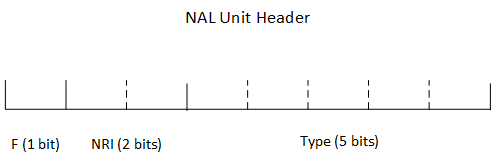
\includegraphics[width=0.7\linewidth]{NALUnitHeader.png}
\caption{NAL Unit Header Structure}
\label{fig:NALHeaderStructure}
\end{figure}
The fields of the header are designated as follows:
\begin{itemize}
\item F: forbidden bit; should always be 0
\item NRI: used to indicate if the content of this NAL unit should be used to reconstruct reference pictures in inter picture prediction
\item Type: Specifies the NAL unit payload type
\end{itemize}

Important types of NAL units are different parameter sets that contain relevant information about a given video stream or frame. These can be broken down into sequence parameter sets and picture parameter sets. The sequence parameter set can be transmitted well in advance of the actual video stream and allow robust protection against the loss of information that changes infrequently during a specific session. Picture parameter sets contain relevant information that remains unchanged for a particular coded picture. Following the NAL unit is the VCL coded frames which the decoder will process based on the type of NAL unit. The H.264/AVC specification also defines a set of profiles and levels which specify different sets of required functional support for decoders. They are designed to support a high degree of interoperability between various different applications of the standard. According to \cite{H264AVCOverview}, ``A profile defines a set of coding tools or algorithms that can be used in generating a conforming bit-stream, whereas a level places constraints on certain key parameters of the bitstream.'' There exist a number of profiles which provide various features and varying amounts of flexibility and customization points. Some examples of profiles and their applications are:
\begin{itemize}
\item Constrained Baseline Profile: low cost applications such as video conferencing in mobile
\item Baseline Profile: used in video conferencing
\item Main Profile: used in various mainstream broadcast and storage applications
\item  Extended Profile: intended to be used as a streaming profile
\item  High Profile: broadcast and disk storage applications (HDTV, Blu-ray, etc.)
\end{itemize}
For video conferencing applications or streaming from mobile devices such as the system proposed in this paper the constrained baseline or baseline profile are appropriate choices. More detailed information on profile types and their constraints can be found in section A.2 of \cite{H264Spec}.

In this study, video frames are encoded using the constrained baseline profile. Thus, we have the most basic set of features and can only encode I and P frames (there is no B frame support for this profile) \cite{H264Spec}. The type of data being transmitted can be determined based on the NAL unit header. Figure \ref{fig:H264PacketFormat}3 shows how each packet is formatted in the system presented here.
\begin{figure}[h]
\centering
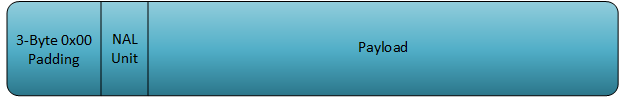
\includegraphics[width=0.8\linewidth]{H264HeaderFormat.png}
\caption{H.264 Packet Format}
\label{fig:H264PacketFormat}
\end{figure}
Every packet is padded with three bytes of 0x00. This is immediately followed by the NAL unit for that frame. Finally, we have the encoded data. In the NAL unit, the very first byte is the NAL unit header. In this study, three types of NAL units are defined based on the NAL unit header:
\begin{itemize}
\item 0x67: This packet contains a sequence parameter set for the next segment of video
\item 0x61: This packet contains the next I-Frame
\item 0x41: This packet contains a P-Frame
\end{itemize}
Using NAL header, one can determine when a new segment of video is started and weigh the relative importance of each incoming packet. 

In the next section, we will discuss the scalable video coding extension of H.264 and compare it with the cognitive parameter adaptation method propsed in this paper.

In the next section, we will discuss the scalable video coding extension of H.264 and compare it with the method of encoding parameter adaptation that we are using to achieve video bandwidth control.

%%%%%%%%%%%%%%%%%%%%%%%%%%%%%%%%%%%%%%%%%%%%%%%%%%%%%%%%%%

\section{Scalable Video Coding vs. Single Layer Video Streams}
\label{sec:SVC}

A major concern in video streaming systems is uncertain channel conditions affecting the quality of the video stream. For example, when transmitting a stream at a certain quality with a video bandwidth $B$ over a congested channel where the channel bandwidth $C$ fluctuates such that $C < B$, the receiving terminal may experience significant degradation of video quality. In order to combat this, scalable codecs have been developed which can alter a certain resolution of the video to fit the channel. This alteration is made to the temporal or spatial resolution of the video or the quality. In H.264/SVC, this is accomplished by removing certain parts of the bit stream in such a way that the underlying streams still represent a valid bit stream for the decoder \cite{SVCOverview}. For example, a transmitter may send one base layer bit stream and multiple enhancement layer bit streams with the receiver selecting which of these to send to the decoder. In this, video bandwidth can be controlled by choosing only the necessary bit streams to stay within the channel bandwidth. Contrast this with a single layer video stream in which a single bit stream is transmitted which represents a valid stream for a given decoder. In order to have control over the bandwidth of the video, the transmitter must encode the source video with different encoding parameters and the receiving decoder must be able to adapt to these changes. We will compare these two methods of adapting a video stream to varying channel conditions; first, the Scalable Video Coding extension of H.264 as described in \cite{SVCOverview}, and second, using a single layer video stream and altering encoding parameters at the source. 

The Scalable Video Coding extension of H.264/AVC inherits all of the base functionality of H.264 with only the necessary added features to achieve scalable video streaming. In this, it supports the primary scalability parameters, being temporal, spatial, and quality resolution. To achieve temporal scalability, the transmitter may send multiple temporal streams divided into a temporal base layer and one or more temporal enhancement layers \cite{SVCOverview}. One may label these streams as $T_0$ through $T_k$. A receiving decoder then simply needs to know which of these access units are valid or invalid for the current stream, starting from $0$ through $n$ where $n\le{k}$. The ability to partition a stream as such and play only the valid streams is already present in the H.264/AVC standard with the employment of reference picture memory control \cite{SVCOverview}. The partitioning of a stream into multiple temporal streams is illustrated in Figure \ref{fig:SVCTemporalScaling}.
\begin{figure}[h]
\centering
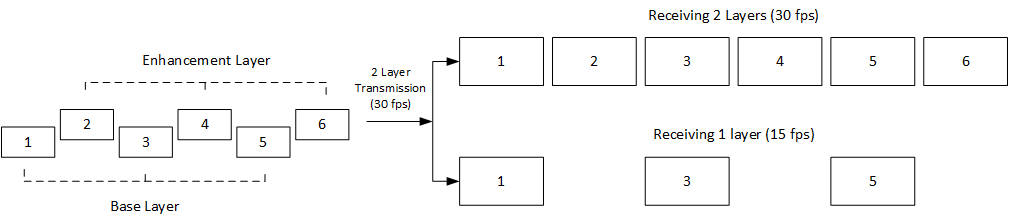
\includegraphics[width=0.8\linewidth]{SVCTemporalScalability.png}
\caption{Temporal Scalability with H.264/SVC \cite{SVCOverview}}
\label{fig:SVCTemporalScaling}
\end{figure}
In order to achieve spatial scalability, SVC uses multi-layer coding with inter-layer prediction \cite{SVCOverview}. Multiple layers are transmitted, each corresponding to a specific spatial resolution and referred to by an integer valued dependency identifier between $0$ and $d-1 $where $d$ is the number of spatial layers \cite{SVCOverview}. Quality scalability works on the same principle as spatial scalability with the layers transmitted being of the same spatial resolution. 

Another method to control the bandwidth of a video stream is to use single-layer coding and manipulate the encoding parameters at the source. In a single-layer coded video stream, one bit stream is encoded and sent to the receiver. This bit stream is of a fixed spatial, temporal, and quality resolution for the entire sequence of video. There is no mechanism built in to the codec to change spatial, temporal, or quality resolution midstream. In this, one can control the bandwidth of the video by using different encoding parameters at the source for different segments of video. We can partition a video stream into multiple segments (sequences) labeled $T_k,k=0\ldots{n-1}$ where $n$ is the number of segments for the given session and $T_k$ is the time instance when the segment $k$ begins. Such a partitioning may be known in advance or can be determined as a function of the channel bandwidth if channel bandwidth can be measured with some reasonable degree of accuracy; for example, using a method like DIChirp as laid out in \cite{DIChirp}. At each time instance $T_k$, the transmitter resets the encoding parameters in such a way that the bandwidth of the video is altered to fit to the channel. When this occurs, a new sequence parameter set is introduced into the stream to signal the changes to the encoded video to the decoder. A sample stream is depicted in Figure \ref{fig:SingleLayerSwitching}.
\begin{figure}[h]
\centering
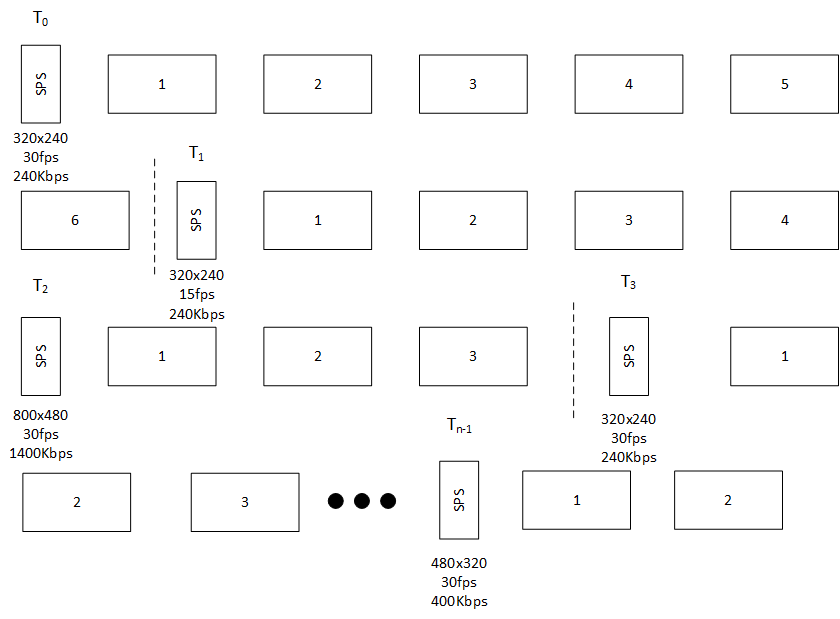
\includegraphics[width=0.8\linewidth]{SingleLayerParameterSwitching.png}
\caption{Single Layer Encoder Parameter Switching}
\label{fig:SingleLayerSwitching}
\end{figure}
The changes to the encoding parameters will insert a delay into the stream for the time it takes to restart the encoding process. To compensate for this delay and to handle the alteration events at time $T_k$, we propose the receiver architecture in Figure \ref{fig:ReceiverArchitecture}.
\begin{figure}[h]
\centering
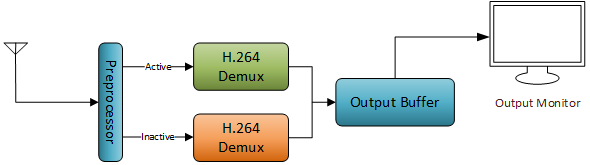
\includegraphics[width=0.8\linewidth]{ReceiverArchitecture.png}
\caption{Receiver Architecture}
\label{fig:ReceiverArchitecture}
\end{figure}
In the proposed receiver architecture, we employed a preprocessor which inspects the NAL unit headers of each incoming packet and determines if and when the video stream has changed. In this implementation, a new stream arrives when the NAL unit header is 0x67. At this event, the idle decoder thread will be invoked and set up to decode the next sequence of video. The previously active decoder thread empties its queue prior to the start of the new segment of video. When the active thread signals completion, the new thread takes over.

In our system, we decided to use a single layer video stream with the receiver architecture in Figure \ref{fig:ReceiverArchitecture} to achieve video bandwidth control. We are able to accomplish this by using a hardware based H.264/AVC encoder. As a result, we are able to initialize the encoder in real time and there is no CPU overhead when it comes to encoding frames (vs. a software encoder). In addition, this real-time efficiency allows us to achieve rapid encoding parameter switches resulting in minimal delay between video segments. We can control the temporal, spatial, and quality resolution of each video segment, effectively allowing us to control the bandwidth of the video with a range of scalability options. 

In our system, we decided to use a single layer video stream with the architecture proposed in Figure 6 to achieve video bandwidth control. We are able to accomplish this by using hardware based video codecs; in particular, a hardware H.264/AVC encoder. As a result, we are able to initialize the encoder in real time and there is no CPU overhead when it comes to encoding frames (vs. a software encoder). In addition, this real-time efficiency allows us to achieve rapid encoding parameter switches resulting in minimal delay between video segments. We can control the temporal, spatial, and quality resolution of each video segment, effectively allowing us to control the bandwidth of the video with a range of effects of the output.

%%%%%%%%%%%%%%%%%%%%%%%%%%%%%%%%%%%%%%%%%%%%%%%%%%%%%%%%%%

\section{System Architecture}
\label{sec:Architecture}
\begin{figure}[h]
\centering
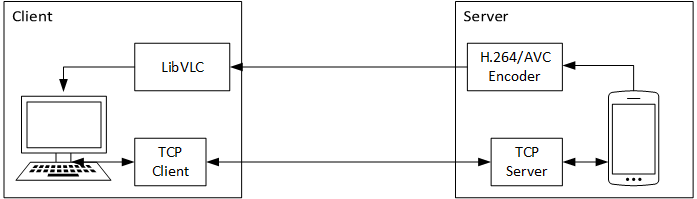
\includegraphics[width=0.8\linewidth]{SystemArchitecture.png}
\caption{System Architecture}
\label{fig:SystemArchitecture}
\end{figure}

A basic outline of our system architecture is depicted in Figure \ref{fig:SystemArchitecture}, with the streaming clients, streaming server, and constituent components. The camera system that we have developed consists of a video client and a streaming server. The client connects to the server to request a new streaming session, displaying the video in a media player based on the VideoLAN VLC player. The streaming server is an Android application implemented on Qualcomm MSM8960 hardware. Video is encoded on the device using a hardware H.264/AVC encoder and streamed to the client using raw UDP packets. We decided to deliver video without a higher level wrapper protocol (such as the Real-time Transfer Protocol (RTP) \cite{RTP} or the Real-Time Streaming Protocol (RTSP) \cite{RTSP}). The server is designed to send a unicast stream to the client connected to it, and a client can view any number of video streams from different servers. The client and server design is detailed in the following sections.

\subsection{Client Design}

The client, implemented as a desktop application, consists of a control center and one or more video windows. The video windows contain a media player for displaying the video, as well as necessary controls for the user to manipulate any of the encoding parameters of the stream. 

The media player uses LibVLC, a library used in the popular VLC media player developed by the VideoLAN group. In the media player, we encapsulate the main functionality for configuring the player and playing a certain stream.  The media player is configured to be consistent with the architecture described in section \ref{sec:NALandPacketization} of this paper. Through configuration of the media player back end, we set up two decoder threads that are used to demultiplex a video stream. This allows us to dynamically change the encoding parameters midstream without seeing a significant effect on video playback. We can then control the bandwidth of the video while still maintaining an optimal user experience. In order to play the video itself, we point the media player to the MRL `\verb=udp/h264://@:[port_num]='. This MRL specifies a raw UDP stream that can be demultiplexed using H.264/AVC. The value of ``\verb=port_num=''  is configured to the port to which video is being streamed to.

On top of the media player is a TCP client that provides interaction with the server. When a new video stream is requested, the client attempts to connect to the server, and upon successful connection, is starts the media player. This client then sends all requests to the server and reacts appropriately to responses.

The client is responsible for determining the correct choice of encoding parameters and for managing the bandwidth of the video based on the bandwidth of channel. In this, the client is equipped with the necessary tools to determine the current channel bandwidth and respond to changes appropriately. These decisions should be based on the user's preferences (if an accurate model of the user’s preferences has been developed) or resort to a default decision function (when learning the user’s preferences). The client should also be smart enough not to interfere with the user when they make their own decisions about how to scale the video. The method by which we develop user profiles and utilize them will be discussed in section \ref{sec:UserProfiles} of this study.

\subsection{Server Design}

Our camera server application runs on a DragonBoard APQ8060A development board utilizing a Qualcomm APQ8060A processor. The application captures live video from an 8MP camera, at varying spatial and temporal resolutions. A TCP server handles all incoming connections from clients and services any requests. On each connection request, a new thread is forked that acts as an interface between the client and server. A handle to the encoder is given to each of these threads to allow them control over the resolutions of the video streams. The handle is encapsulated in an object we call the ``encoder activation interface''. This object, as the name implies, acts as an interface to the encoder (as well as the camera). Via this interface a consumer may initialize, destroy, and alter an encoder for a certain video stream. This allows the clients full control over the parameters of the video and enables it to control the video bandwidth. The server remains agnostic of channel conditions and acts as a slave to the connected clients, reconfiguring the stream as necessary for each request. The reasoning behind this is that the client application learns the user’s preferences and therefore makes more intelligent decisions about the encoding parameters than the server.

\subsection{Session Management}

The system contains a communication layer using TCP for messaging between the client and server. This communication layer acts as a session manager. TCP is used for reliable communication of messages between terminals as well as to signal the beginning and end of a streaming session. A streaming session begins once the server accepts a client's connection, and ends when one of the terminals disconnects. When a client wishes to receive a particular stream from a particular server, it first attempts to make a connection with the server. Upon connection, the server initializes a new thread to service the client’s requests. The server thread first starts the encoder, which begins streaming packets containing the encoded H.264 frames. This thread then enters a loop in which it responds to the client's requests until it detects that the client has disconnected. We have defined a very simple protocol for submitting such requests in which the client either requests to alter encoding parameters or stop the video stream. The request to update encoding parameters also serves to start a stream again if it has been previously stopped. To update the encoder, the client sends the following message:
%\lstinputlisting{start.xml}
\begin{lstlisting}[language=xml, frame=single]
<request action="start">
	<width>#</width>
	<height>#</height>
	<fps>#</fps>
	<rate>#</rate>
</request>
\end{lstlisting}
where ``width'' is the new desired width, ``height'' is the new desired height, ``fps'' is the new desired frame rate, and ``rate'' is the new desired video bitrate. To stop the encoder, the following message is sent with the request action as stop:
%\lstinputlisting{stop.xml}
\begin{lstlisting}[language=xml, frame=single]
<request action="stop" />
\end{lstlisting}
Upon disconnecting, the thread processing the client's requests will shut down the encoder, stop the video stream, and exit.

%%%%%%%%%%%%%%%%%%%%%%%%%%%%%%%%%%%%%%%%%%%%%%%%%%%%%%%%%%

\section{Snapdragon Video Framework}
\label{sec:Snapdragon}

The DragonBoard APQ8060A is equipped with numerous hardware based codecs for both audio and video. We decided to use the hardware encoder in order to encode frames in real time. In addition, the extra speed we acquire greatly assists in our video scaling method. We will now describe how the camera server works to capture video frames, encode them, and send them as raw UDP packets.

To access the hardware components, Android provides a wrapper to the OpenMAX Integration Layer called IOMX which can interact with and utilize hardware media codecs. The OpenMAX Integration Layer is a component based API designed to provide a layer of abstraction on top of multimedia hardware and software architecture. It is also designed to give media components portability across a range of devices. Figure \ref{fig:OpenMAX} illustrates the various layers designed in OpenMAX. 
\begin{figure}[h]
\centering
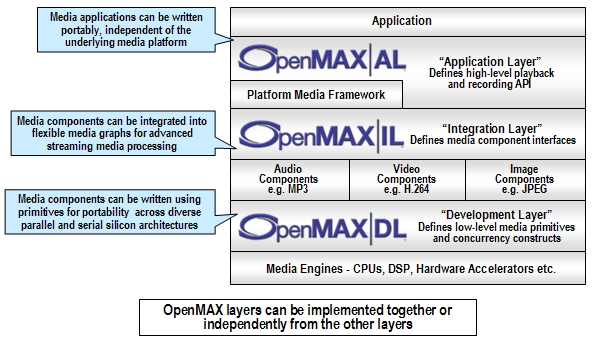
\includegraphics[width=0.5\linewidth]{openmax.png}
\caption{OpenMAX Layers}
\label{fig:OpenMAX}
\end{figure}

With the introduction of the stagefright media framework (Figure \ref{fig:Stagefright}), Google added the OpenMAX IL functionality to the Android operating system, allowing OEMs the ability to provide software hooks that serve as an interface to the hardware for developers.
\begin{figure}[h]
\centering
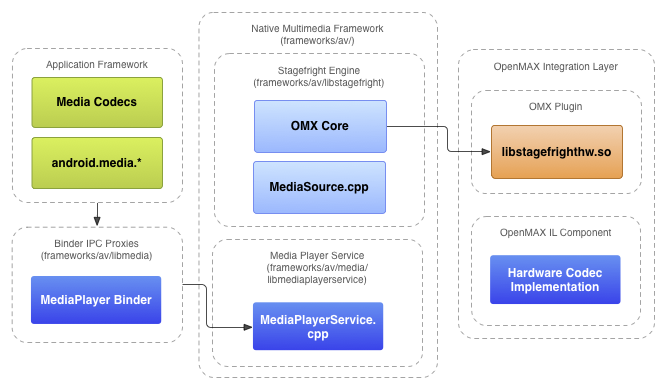
\includegraphics[width=0.5\linewidth]{stagefright.png}
\caption{Stagefright Media Framework}
\label{fig:Stagefright}
\end{figure}

In addition, Qualcomm has developed and provided a sample API that utilizes IOMX to encode and decode various audio and video formats. Our server is leveraging this API to interact with the hardware H.264/AVC encoder present on the device. Qualcomm's implementation can be broken down into a few different levels, as depicted in Figure \ref{fig:QualcommAPI}. The lowest levels are the hardware, OpenMAX IL, and IOMX. The API consists of C++ classes which wrap around IOMX, as well as a public interface written in C, providing ease of use for higher level code. In this, one can query available codecs, activate and initialize a session, encode/decode frames, and perform cleanup when a session ends.
\begin{figure}[h]
\centering
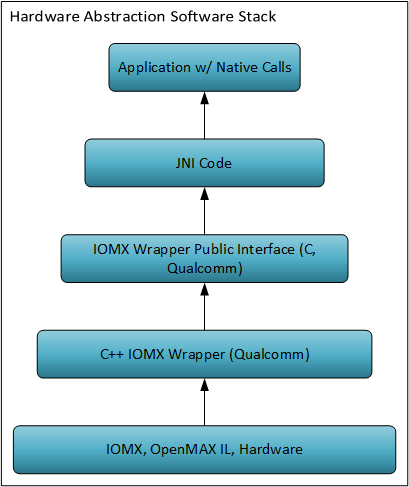
\includegraphics[width=0.4\linewidth]{QualcommAPI.png}
\caption{Encoder Hardware Abstraction}
\label{fig:QualcommAPI}
\end{figure}
In this study, the Qualcomm API is used in an Android application via the Java Native Interface (JNI) which enables interaction with the public interface of the API. The application developed in this study utilizes this API to quickly and efficiently encode video in real time. In addition, the activation and tear down of an encoding session occurs with very minimal delay.

%%%%%%%%%%%%%%%%%%%%%%%%%%%%%%%%%%%%%%%%%%%%%%%%%%%%%%%%%%

\section{User Profiles and Bandwidth Optimization}
\label{sec:UserProfiles}

The development of user profiles allows the client to make intelligent scaling decisions in line with how the user would have changed the video. This relieves the burden on the user to figure out how video should be scaled in different contexts, making it critical for a widely acceptable system. The learning and prediction mechanism proposed in this study offers a simple, yet effective way to provide dynamically adaptive video streams tailored to each individual.

\subsection{Preferences and Profiles}
We develop a profile of the user which will determine how video will be scaled when it is no longer optimized to the transmission channel. In this, we have designated the user to belong to one of four discrete classes which represent their preferences in relation to video quality:
\begin{itemize}
\item Class 0: User prefers high temporal and spatial resolution, no quality preference.
\item Class 1: User prefers high temporal resolution; optimize spatial resolution for quality.
\item Class 2: User prefers high spatial resolution; optimize temporal resolution for quality.
\item Class 3: User prefers optimal quality; configure temporal and spatial resolution appropriately.
\end{itemize}
Knowing these preferences, we optimize the video bandwidth by weighing the video resolutions with higher or lower priority. This translates into the client treating lower priority parameters more harshly when determining the new encoding parameters.

Transforming these classes to their equivalent binary form we can represent them with a 2 bit value in which the first bit conveys the temporal resolution preference and the second bit conveys the spatial resolution preference. A set bit indicates the desire for a high weight given to this resolution at the expense of quality, and an unset bit indicates the desire to optimize quality resolution at the expense of the resolution in question. In this, we can find the best way to alter the spatial and temporal resolution such that the video bandwidth will fit the channel and align with the user's desires in terms of quality. The creation of these user profiles is accomplished using machine learning; in particular, by solving the classification problem using support vector machines.

\subsection{Creating User Profiles}
In order to create a profile for each user, we employed a supervised learning algorithm to create a decision function based on the user’s behavior to predict the class a user falls into. The decision function is calculated using the LibSVM implementation of a C support vector machine with a radial basis kernel \cite{LibSVM}.

In supervised machine learning, a training set composed of a series of training samples is presented as input to the learning algorithm, the output of which is a set of coefficients for a decision function. In classification problems such as ours, the training samples are the values of a set of contextual features which we find relevant to the output, and a label for each of these vectors which denotes what class applies at the instant of the sample. The features used in this study are the channel bandwidth and the content type of the video (i.e. high quality medical, talking head, sporting event, etc.). For the two preferences being learned we use two C support vector machines with radial basis kernels. The C support vector machine classification algorithm used in this study is defined in \cite{LibSVM}. To use support vector machines to learn user preferences, we can define a training set as a feature vector $x_i \in \mathbf{R^n}  ,i=1\ldots{l}$ and the class label vector $y_i \in \lbrace 1,-1 \rbrace $ where 1 and -1 indicate the two distinct classes. The primal optimization problem in equation (\ref{equ:PrimalOpt}) is then defined in \cite{LibSVM}
\begin{equation}
\begin{aligned}
\label{equ:PrimalOpt}
& \underset{w,b,\xi}{\text{minimize}}
& & \frac{1}{2}w^Tw+C\sum_{i=1}^{l} \xi_i \\
& \text{subject to}
& &  y_i(w^T\phi(x_i) + b) \ge 1 - \xi_i
\end{aligned}
\end{equation}
\[ \xi_i \ge 0, i = 1,\ldots ,l \]
where $\phi (x_i)$ maps $x_i$ into higher dimensional space and $C > 0$ is a configurable parameter \cite{LibSVM}.The dual problem presented in equation (\ref{equ:DualProb}) can then be solved in order to account for the possible high dimensionality of the vector parameter $w$.
\begin{equation}
\begin{aligned}
\label{equ:DualProb}
& \underset{\alpha}{\text{minimize}}
& & \frac{1}{2}\alpha^TQ\alpha-e^T\alpha \\
& \text{subject to}
& &  y^T\alpha = 0
\end{aligned}
\end{equation}
\[ 0 \le \alpha_i \le C, i = 1,\ldots ,l \]
where $e$ is a column vector of all ones, $Q_(i,j)=y_i y_j K(x_i,x_j)$ and $K(x_i,x_j ) \equiv \phi (x_i )^T \phi (x_j)$ is the radial basis function (RBF). The RBF $K$ is a Gaussian distribution, defined in equation (\ref{equ:Gaussian}).
\begin{equation}
\label{equ:Gaussian}
K(x_i, x_j) = e^{-\gamma ||x_i - x_j||^{2}}
\end{equation}
where $\gamma$ is a configurable parameter selected by the user. Finally, the optimal $w$ is computed using equation (\ref{equ:W}), and the decision function is defined by equation (\ref{equ:DecisionFunction}).
\begin{equation}
\label{equ:W}
w = \sum_{i=1}^{l} y_i \alpha_i \phi (x_i)
\end{equation}
\begin{equation}
\label{equ:DecisionFunction}
sgn(w^T\phi (x) + b) = sgn(\sum_{i=1}^{l} y_i\alpha_i K(x_i, x_j) +b)
\end{equation}
If we consider the graphical representation of $x_i$ and $y_i$, we have a multidimensional input space and class labels associated with each vector from $x$. The support vector machine attempts to find a hyperplane that separates the two classes with the widest margin, using kernels to support nonlinear separations. From this hyperplane we obtain a decision function that is used to predict class labels for new input vectors. In this study, we train the support vector machines to predict the user’s preferences using a combination of implicit and explicit feedback. 

When a new user begins interacting with the system, they are initiated in ``learning mode.'' In learning mode, a change in channel bandwidth will result in a knee-jerk reaction by the system to simply alter the quality resolution of the video, leaving spatial and temporal resolution unchanged. Explicit feedback is obtained from the user. The user's interaction with the system is recorded and forms the training data set for the support vector machines. When the training set is sufficiently large enough to accurately train the support vector machines, 3-fold cross validation is performed to ensure accurate selection of $C$ in equation (\ref{equ:PrimalOpt}) and $\gamma$ in equation (\ref{equ:Gaussian}) \cite{LibSVM}. From this, a decision function is created which we use to make predictions. The explicit feedback process is shown in Figure \ref{fig:Feedback}.
\begin{figure}[h]
\centering
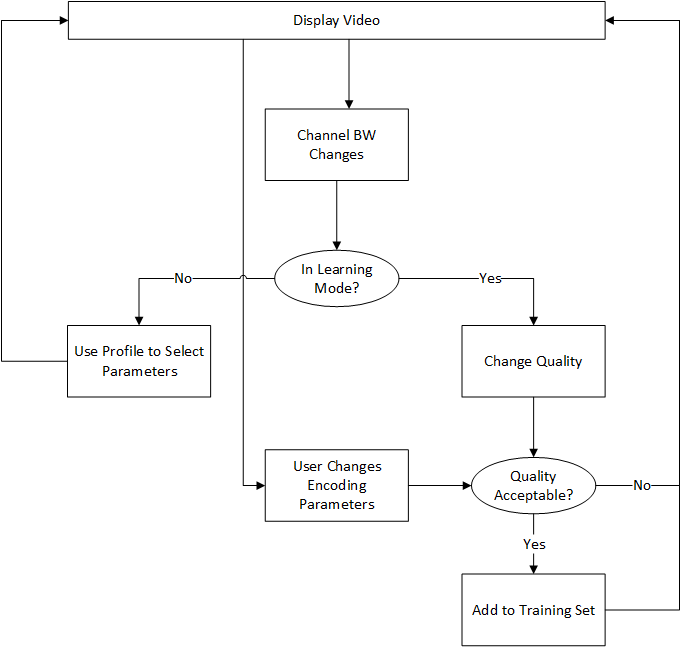
\includegraphics[width=0.5\linewidth]{BandwidthChangeDecisionTree.png}
\caption{Feedback Process}
\label{fig:Feedback}
\end{figure}

\subsection{Video Bandwidth Determinations}
The catalyst for video bandwidth recalculation is when the channel conditions have changed significantly enough to warrant scaling the video. Several methods, such as DIChirp \cite{DIChirp}, have been shown to estimate the bandwidth of the channel within a high degree of accuracy. We will now lay out how changing the various video resolutions will affect the video bandwidth in our system.

In order to alter the quality resolution we change the compression bitrate of the video. The maximum bitrate can simply be calculated as a function of the known channel bandwidth and an optimization constant:
\begin{equation}
\label{equ:BitrateCalculation}
Bitrate_{max} = Bandwidth_{channel} * K
\end{equation}
where $Bitrate_{max}$  is the maximum allowable bitrate, $Bandwidth_{channel}$ is the bandwidth of the channel, and $K$ is the optimization constant determining the percentage of available bandwidth that is acceptable to fill. Due to limitations in our encoder, the max bitrate must be calculated as a function of the frame rate. We are using the following calculation: 
\begin{equation}
\label{equ:LimitedBitrateCalculation}
Bitrate_{max} = \frac {Bandwidth_{channel}}{\frac {T} {17.28} } * K
\end{equation}
where $T$ is the frame rate of the video. We can then find an optimal bitrate for a given spatial resolution as a function of the video dimensions and an optimization constant:
\begin{equation}
\label{equ:OptimalBitrate}
Bitrate_{opt} = width * height * Q_{max}
\end{equation}
where $width$ and $height$ are the dimensions of the video, and $Q_{max}$ is the optimization constant which can be configured to find the highest necessary bitrate to deliver high quality video at a given spatial resolution. The output bitrate is then simply $Bitrate_{max}$ unless we wish to be conservative with channel bandwidth. In this case, the best choice of bitrate is either the maximum allowable bitrate or maximum necessary bitrate for the given channel, spatial resolution, and temporal resolution. We can select from equations (\ref{equ:SelectMaxBitrate}) and (\ref{equ:OutputBitrate}) when determining which output bitrate to use.
\begin{equation}
\label{equ:SelectMaxBitrate}
Bitrate_{out} = Bitrate_{max}
\end{equation}
\begin{equation}
\label{equ:OutputBitrate}
Bitrate_{out} = \min (Bitrate_{max} , Bitrate_{opt})
\end{equation}
The highest necessary bitrate for delivering the best possible quality to the client is given in equation (\ref{equ:OutputBitrate}).

Determining the temporal and spatial resolution will affect the quality resolution such that higher values will result in lower quality once the bitrate has reached $Bitrate_{max}$. We inspect the user’s class in order to set these two parameters, as the class tells us if the temporal/spatial resolution should be optimized or if the quality should be optimized. In this study, we limit the possible temporal resolution values to 30 and 15. In the case where the temporal resolution bit is set in the user’s class, we simply set the frame rate to 30 fps, and if unset, we change the frame rate to 15 fps. If the spatial resolution bit is set, the spatial resolution is changed to the maximum value. When the bit is unset, we first calculate $Bitrate_{max}$, then reduce the spatial resolution until:
\begin{equation}
\label{equ:OptMaxRelation}
Bitrate_{opt} \le Bitrate_{max}
\end{equation}
This will result in a spatial resolution that will be small enough to provide optimal quality video.

\subsection{Scaling Decisions}

The way that video bandwidth is optimized depends on the class that the user falls into for the given feature set at the time $T_k$ (the moment when the encoding parameters of the $k^{th}$ segment of video are selected). When channel bandwidth changes significantly enough, the first action we take is to predict the user’s preferences using the two decision functions we have already generated. This provides us with a bitmask that serves as the user’s class; the primary purpose of this class is to specify the order in which to scale the encoding parameters. This ordering also depends on whether or not the video bandwidth is increasing or decreasing. The chart given in Figure \ref{fig:ScalingDecisionChart} depicts the possible decisions that can be made about the video bandwidth.
\begin{figure}[h]
\centering
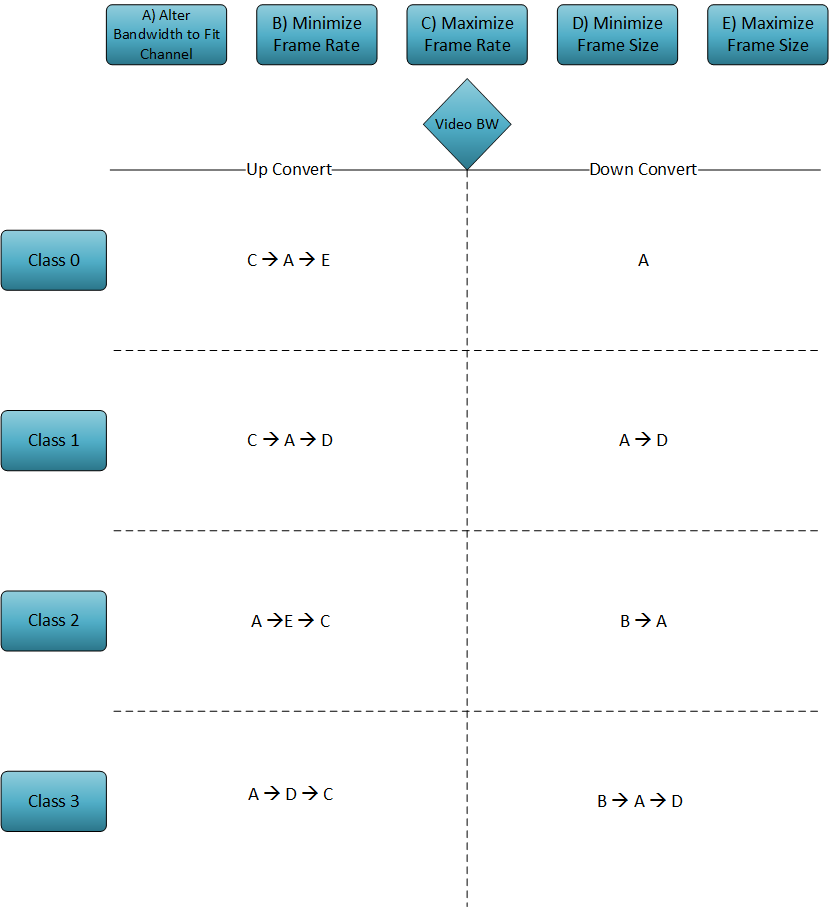
\includegraphics[width=0.7\linewidth]{BandwidthDecisions.png}
\caption{Bandwidth Decisions}
\label{fig:ScalingDecisionChart}
\end{figure}
We can then successfully adapt to channel bandwidth changes and alter the encoding parameters in such a way that the user’s desires are fulfilled.
%%%%%%%%%%%%%%%%%%%%%%%%%%%%%%%%%%%%%%%%%%%%%%%%%%%%%%%%%%

\section{Experimental Results}
\label{sec:Results}

To validate the cognitive video scaling solution, we have developed a test bed as shown in Figure \ref{fig:Testbed}.
\begin{figure}[h]
\centering
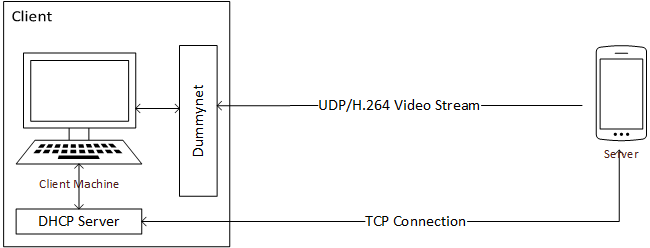
\includegraphics[width=0.5\linewidth]{CameraSystemTestbed.png}
\caption{Camera System Test Bed}
\label{fig:Testbed}
\end{figure}
We created a point to point connection between the client and server by setting up the client machine as a DHCP server and connecting it directly to the embedded video server, allocating it an IP address on an arbitrary subnet. We are using dummynet , a widely used network emulator, to emulate the behavior of internet in the lab environment. With dummynet, one can control the traffic over a specific channel by limiting bandwidth, inserting packet losses, inserting delay, etc. In order to simulate bandwidth change detection the client simply reads from a file that contains channel bandwidth information. In our test set up we developed a test application which simultaneously sets the bandwidth of the channel to varying values at certain intervals using dummynet, and writes this bandwidth to a flat file that the client can read from. With this, we are able to implement some of the conditions of a real network and be aware of the bandwidth in the client application. 

The first experiment tests the ability of the system to control the bandwidth of the video by altering the spatial resolution. Channel bandwidth is kept constant, as well as frame rate which is kept at 30 frames per second. The spatial resolution is changed from 800x480 to 480x320 to 320x240. We used Wireshark to capture and display the bandwidth of the video, obtaining results in Figure \ref{fig:SpatialTest}.
\begin{figure}[h]
\centering
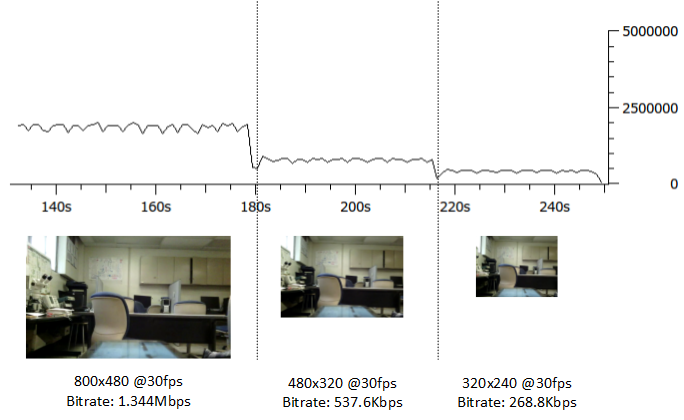
\includegraphics[width=0.5\linewidth]{SpatialResolutionTest.png}
\caption{Spatial Resolution Experiment}
\label{fig:SpatialTest}
\end{figure}
As the spatial resolution is changed, the bandwidth of the video changes accordingly. One can easily deduce that this change is directly proportional to the change in resolution. For example, when the spatial resolution changes from 800x480 to 480x320, the total pixel ratio and the ratio of video bandwidth are equivalent:
\[ \frac{480 * 320}{800 * 480} = \frac{76800}{384000} = 0.4 \]
\[ \frac{537.6Kbps}{1344Kbps} = 0.4 \]
These results indicate that we have successfully demonstrated control over the video bandwidth by altering the spatial resolution of the video. 

In our next test, we showed that we can control video bitrate by altering the amount of compression (number of bits per pixel), resulting in a change in video quality. We tested the system’s response to changes in channel bandwidth by altering the bandwidth from 1600Kbps to 800Kbps to 400Kbps. Spatial resolution was kept constant at 800x400 and temporal resolution was kept constant at 30 fps. The resulting changes in video bitrate, as well as playback quality, are depicted in Figure \ref{fig:QualityTest}.
\begin{figure}[h]
\centering
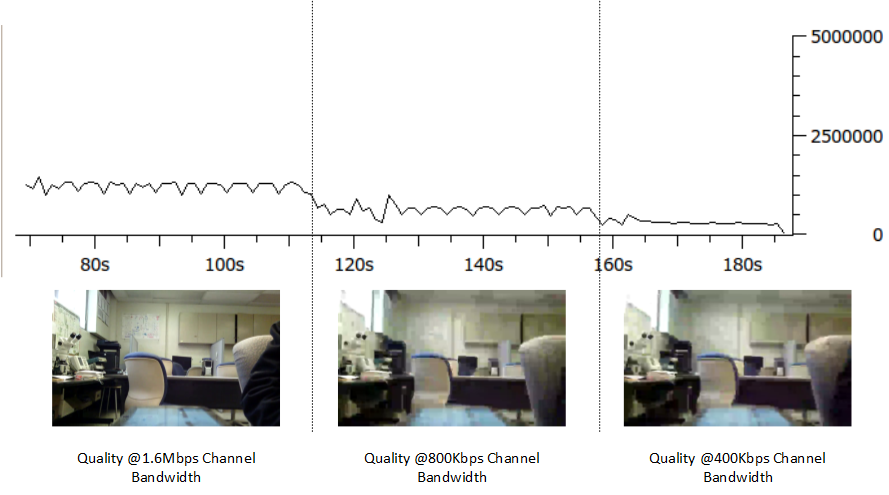
\includegraphics[width=0.5\linewidth]{QualityResolutionTest.png}
\caption{Quality Resolution Experiment}
\label{fig:QualityTest}
\end{figure}
As can be seen from Figure 15, the system successfully and immediately responds to changes in channel bandwidth by reducing the quality resolution of the video. In addition, the reduction in video bitrate is directly proportional to the reduction in available bandwidth.

Finally, we tested the system’s ability to determine the user’s preferences and scale the video appropriately when channel bandwidth changes. For the purposes of this study, we provided the learning mechanism with an arbitrary training set with the intent to prove the system’s ability to properly learn and make predictions. By using a predefined training set we know in advance what classes should be predicted, allowing us to validate the accuracy of the cognitive mechanism by comparing the experimental predicted values with the expected values. The training set used is given in Table \ref{tab:TrainingSet}.
\begin{table} [h]
\caption{Training Set}
\label{tab:TrainingSet}
\begin{tabular}{c|c|c}
\textbf{Channel Bandwidth (Kbps)}&\textbf{Content Type}&\textbf{Class Label}\\
\hline
1200&0&0\\
1300&0&0\\
800&0&2\\
500&0&3\\
900&0&2\\
300&0&3\\
1100&0&0\\
1300&0&0\\
1500&0&0\\
850&0&2\\
500&1&3\\
1200&1&0\\
600&1&1\\
1300&1&0\\
300&1&3\\
400&1&3\\
800&1&0\\
600&1&1\\
700&1&1\\
1200&2&0\\
500&2&3\\
1200&2&0\\
2000&2&0\\
1300&2&2\\
300&2&3\\
900&2&3\\
1400&2&2\\
1900&2&0\\
700&2&3\\
1200&2&2\\
\end{tabular}
\end{table}
The class distribution for this training set is depicted in Figure \ref{fig:ClassDistribution}.
\begin{figure}[h]
\centering
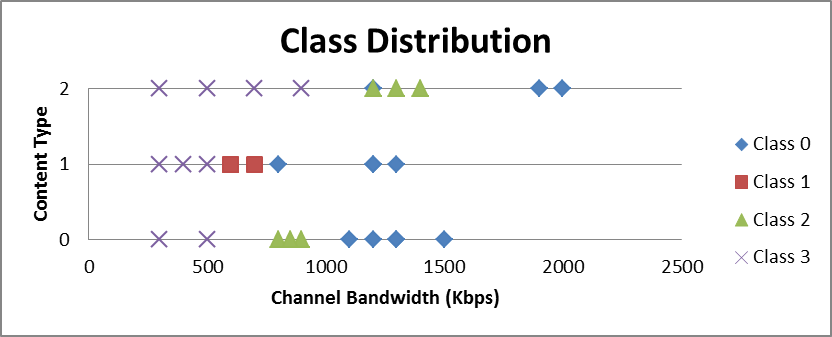
\includegraphics[width=0.5\linewidth]{ClassDistribution.png}
\caption{Class Distribution}
\label{fig:ClassDistribution}
\end{figure}
The ``Content Type'' feature is used to classify different scenes that are transmitted in real world scenarios. For example, a content type of 0 may be a video conferencing application with a ``talking head'' based scene, while a content type of 2 may be a medical based scene that requires extremely high bandwidth and video quality. In this experiment, we used 3 different content types, giving us the approximated expected prediction values in Table \ref{tab:ExpectedValues}.
\begin{table}
\caption{Expected Prediction Values}
\label{tab:ExpectedValues}
\begin{tabular}{c|c|c}
\textbf{Channel Bandwidth (Kbps)}&\textbf{Content Type}&\textbf{Expected Class}\\
\hline
0-500&0&3\\
500-1000&0&2\\
1000+&0&0\\
0-500&1&3\\
500-800&1&0\\
800+&1&0\\
0-900&2&3\\
900-1700&2&2\\
1700+&2&0
\end{tabular}
\end{table}
We trained the support vector machines and tested the learning mechanism by setting the bandwidth to 1600Kbps, 800Kbps, and 400Kbps while viewing video streams with content types 0, 1, and 2. For equation (\ref{equ:BitrateCalculation}) we selected the $K$ parameter to be 0.85 and for equation (\ref{equ:OptimalBitrate}) we selected the $Q_{max}$ parameter to be 3.5. In all the experiments the output bitrates are selected from equation (\ref{equ:SelectMaxBitrate}). The resulting bandwidth changes, encoding parameter changes, and class predictions are given in Figures \ref{fig:TalkingHead}-\ref{fig:Medical}.
\begin{figure}[h]
\centering
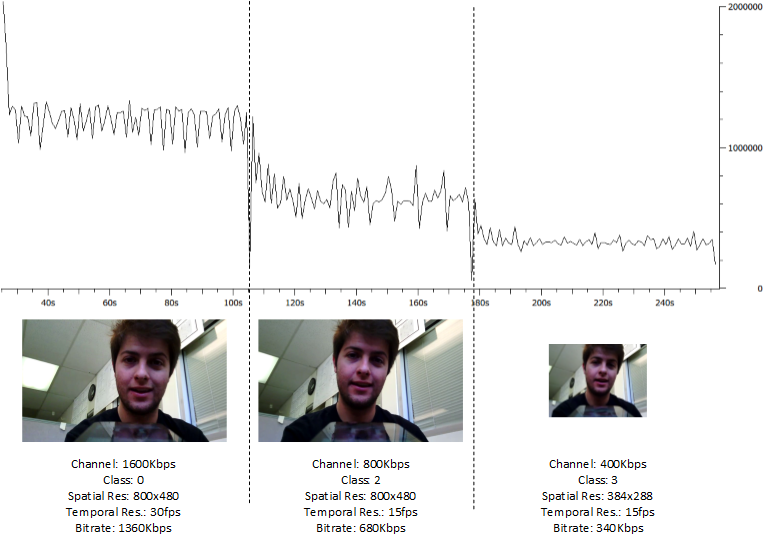
\includegraphics[width=0.5\linewidth]{TrainingExperimentTalkingHead.png}
\caption{Predictions With Content Type 0}
\label{fig:TalkingHead}
\end{figure}
\begin{figure}[h]
\centering
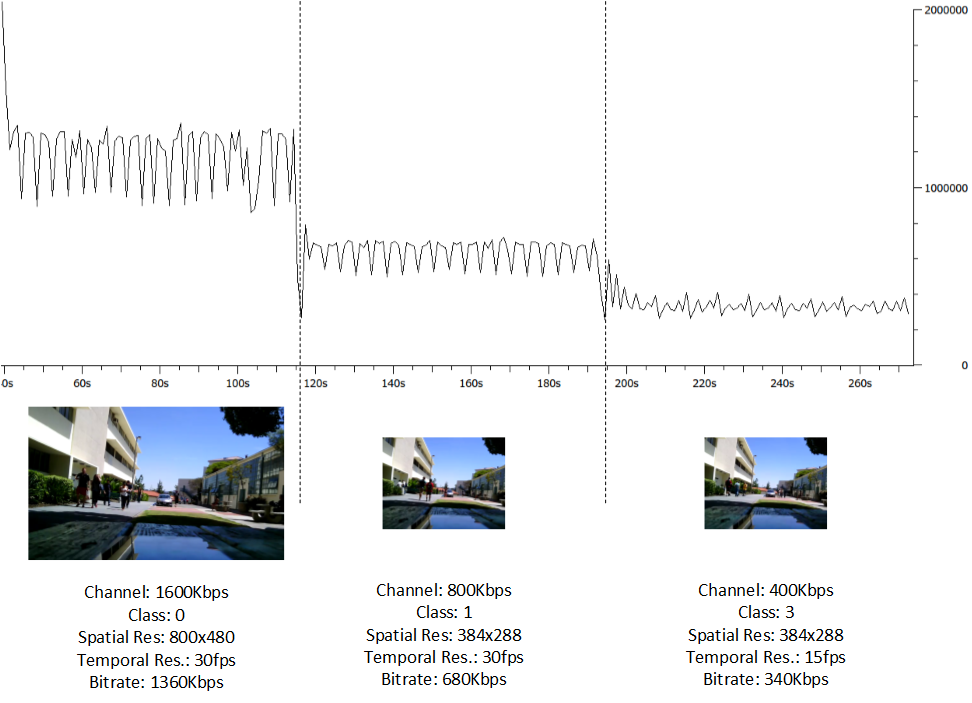
\includegraphics[width=0.5\linewidth]{TrainingExperimentSports.png}
\caption{Predictions With Content Type 1}
\label{fig:Sports}
\end{figure}
\begin{figure}[h]
\centering
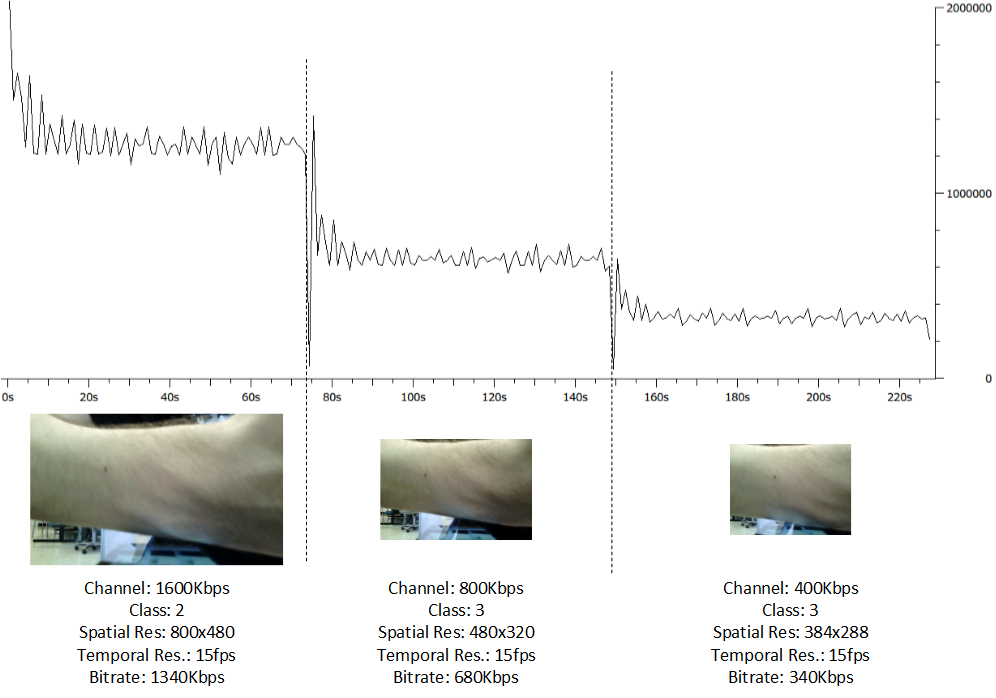
\includegraphics[width=0.5\linewidth]{TrainingExperimentMedical.png}
\caption{Predictions With Content Type 2}
\label{fig:Medical}
\end{figure}
In all cases, the video bandwidth was adapted when the channel bandwidth changed. In addition, the video bandwidth was consistently kept at 85\% of the channel bandwidth as a result of our selection of $K$. In order to validate the accuracy of the predictions, Table \ref{tab:PredictedClasses} compares the expected class values and the predicted class values at time instances $T_0$, $T_1$, and $T_2$, where $T_0$ is the instant when the channel bandwidth changes to 1600Kbps.
\begin{table} [h]
\caption{Expected vs. Predicted Classes}
\label{tab:PredictedClasses}
\begin{tabular}{c|c|c|c}
\textbf{Segment}&\textbf{Content Type}&\textbf{Expected Class}&\textbf{Predicted Class}\\
\hline
&0&0&0\\
$T_0$&1&0&0\\
&2&3&3\\
\hline
&0&2&2\\
$T_1$&1&1&1\\
&2&3&3\\
\hline
&0&3&3\\
$T_2$&1&3&3\\
&2&3&3\\
\end{tabular}
\end{table} 
As the table indicates, the support vector machines predicted the correct class with 100\% accuracy. In addition, the resulting changes to the encoding parameters followed the changes defined in Figure \ref{fig:ScalingDecisionChart}. When class 0 was predicted, the spatial and temporal resolutions were kept high at the cost of fewer bits per pixel. When class 1 was predicted, the temporal resolution was kept high and the spatial resolution was reduced. The prediction of class 2 resulted in a loss in temporal resolution with the spatial resolution being kept high. Finally, when class 3 was predicted, the spatial and temporal resolutions were reduced, resulting in greater quality with more bits per pixel. 
%%%%%%%%%%%%%%%%%%%%%%%%%%%%%%%%%%%%%%%%%%%%%%%%%%%%%%%%%%

\section{Conclusion}
\label{sec:Conclusion}
As the volume of internet traffic related to video streaming increases, the importance of having exceptional bitrate adaptation schemes grows. In addition, these schemes should be aware of not only the channel bandwidth, but the surrounding context of the video being streamed. This context encapsulates the content type of the video, and can extend into other dimensions such as amount of motion, geospatial location, and more. We have presented a solution that takes rate adaptation beyond simply changing the quality of the video when the channel bandwidth becomes limited. Our system determines the user’s preferences about video quality, taking into account if the user prefers a drop in temporal or spatial resolution versus quality resolution. We have demonstrated the ability to adapt to channel bandwidth changes by altering these resolutions. In addition, we have shown that by using support vector machines, we can learn the user’s preferences and successfully adapt the video bandwidth in line with these preferences. Such a system is a viable solution to the changing atmosphere of video providers, contexts, and the increasing and diverse consumer base.

\section*{Acknowledgements}
This study in part has been supported by Qualcomm University program. 


%% The Appendices part is started with the command \appendix;
%% appendix sections are then done as normal sections
%% \appendix

%% \section{}
%% \label{}

%% References
%%
%% Following citation commands can be used in the body text:
%% Usage of \cite is as follows:
%%   \cite{key}         ==>>  [#]
%%   \cite[chap. 2]{key} ==>> [#, chap. 2]
%%

%% References with BibTeX database:

\bibliographystyle{elsarticle-num}
\bibliography{references}

%% Authors are advised to use a BibTeX database file for their reference list.
%% The provided style file elsarticle-num.bst formats references in the required Procedia style

%% For references without a BibTeX database:

% \begin{thebibliography}{00}

%% \bibitem must have the following form:
%%   \bibitem{key}...
%%

% \bibitem{}

% \end{thebibliography}

\end{document}

%%
%% End of file `ecrc-template.tex'. 
